\documentclass[a4paper,12pt]{article}
\usepackage[utf8x]{inputenc}

\usepackage{graphicx}
\usepackage{float}
\usepackage{amssymb,amsmath}
\usepackage{subfig}
\usepackage{url}
\usepackage{rotating}
\usepackage[square, numbers, comma, sort&compress]{natbib}
\usepackage{authblk}
\usepackage{longtable}

\date{08/07/2011}

\begin{document}
 
\section{Project 2: Understanding non-coding Functional RNAs: 
Folding Dynamics and Binding mechanism of Riboswitches}

In order to fully understand the coupling between the ligand binding
and the folding of riboswitch RNAs, we adopt all atomic simulations to
explore this linkage.  We have been engaged in seeking physical
insights into novel ideas that elucidate the interplay between the
Aptamer domain and the Expression domain; this has not been explored
in previous studies.  In particular, we are using very long
time-scales ($>$ 100ns) all-atom multiple MD simulations/trajectories,
to seek an understanding of the role of the branch migration during a
dynamical transition toward the OFF state of S-adenosyl Methione (SAM)
binding riboswitch (SAM-I riboswitch).  Based upon interesting
phenomenon that has been observed in trajectories generated on Ranger,
we have developed new analysis to monitor the trajectory on the
fly. Additionally, these data also provide us the basis of choosing a
system to be submitted for tens of us (microsecond) time scale on
Anton, a machine specially designed for running MD simulations. This
work is being carried out by Wei Huang a final year PhD (expected
graduation Dec 2011) student co-supervised by the PI.  The computing
resources we ask here are critical for our ongoing study on RNA
riboswitch mechanisms.

We need to extend this to cover multiple distinct starting
configuration; the need for multiple trajectories arises because we
have to simulate various initial structures that are sampled by 3D
modeling and thus cover the conformational space appropriately.  In
addition, these multiple all-atom MD simulations should be conducted
with SAM-bound and SAM-free states, since the role of SAM could be
understood by comparing trajectories of two different states.  

Initial work in this project has just been accepted as a Special Issue
of Concurrency and Computing: Practice and Experience (CCPE) for
Emerging Methods for the Life Sciences~\cite{ccpe10}.  The next round
of simulations, should provide conclusive evidence of a potential role
of the SAM in facilitating P1 helix formation over the AT helix
formation, which will eventually clarify whether the proposed branch
migration mechanism as a major switching pathway between two
alternative secondary structures of SAM-I riboswitch.



\section{Project 3: Atomistic Simulations of Physiological Systems}

The long term scientific objective of our project is to develop molecular dynamics simulations of 
medically relevant enzymes into a tool for clinicians to use in determining the cocktail of drugs to 
administer to an HIV-infected individual. This work is supported by grants under EU FP7 and FP6 
via the VPH-NOE (EU FP7-ICT-2007-5.3 223920), Contra Cancrum (EU FP7-ICT-2007-5.3 223979), 
p-Medicine (EU FP7-ICT-2009-6 270089) and CHAIN (EU FP7 HEALTH-2007-2.3.2-7) projects. For such 
applications, reproducible accuracy at the level which can rank drug efficacies, and rapidity 
of acquisition of results (for clinical relevance) are all essential. This takes the application 
of bio-MD techniques into an entirely new domain.

\subsection{Project 3a: Towards patient specific HIV therapy}

\subsubsection{Progress}

The aim of this project is to calculate binding affinities for HIV-1 enzymes with the anti-viral 
drugs used to target them in clinical practice. We have previously shown an excellent ability to
reproduce experimental results for genetic variants of the HIV-1 protease binding the drug 
lopinavir using ensembles of 50 replica simulations of 4 ns trajectory duration \cite{Sadiq2010}. 
Our work during the current grant has focussed on extending the use of the simulation and analysis 
protocol we have developed to the other FDA approved protease inhibitors (PIs -all of the inhibitors 
included in the study are listed in Table \ref{tab:inhibitors}). 
The initial stage of this process is to access the protonation state of the catalytic dyad of the 
protease bound to each of the inhibitors, which has now been achieved for all drugs. As part of this 
stage of the project we developed a submission tool based on SAGA (See Project 5) which allowed us 
to coordinate simulation runs on machines on both the TeraGrid (Ranger) and the EU Distributed 
European Infrastructure for Supercomputing Applications (DEISA) [1]. Having completed our investigation 
of the protonation state used for each inhibitor we performed production binding affinity calculations 
for all of the drugs. Our results produced a promising inter-drug ranking but 
suggested that binding affinities are highly dependent on the initial conformation as well as protonation 
state of the catalytic dyad. It was also observed that results for the inhibitor ritonavir were acutely 
sensitive to the conformation of the aspartic acid at position 30. These observations provide the 
motivation for the future work we will describe in Section \ref{se:hiv_future}.

\begin{table}
\begin{center}
\begin{tabular}{l l}
\textbf{Inhibitor Code} & \textbf{Inhibitor Name}\\
\hline
APV & amprenavir\\
IDV & indinavir\\
LPV & lopinavir\\
NFV & nelfinavir\\
RTV & ritonavir\\
SQV & saquinavir\\
AZV & atazanavir \\
TPV & tipranavir \\
\hline
\end{tabular}
\end{center}
\caption{Code and full names of the HIV-1 protease inhibitors (PIs) investigated.}
\label{tab:inhibitors}
\end{table}

In addition to this progress on the originally proposed simulations, we also extended our previous work 
evaluating the binding affinity of HIV-1 protease mutants to the inhibitor lopinavir. As part of 
a previous collaboration in the EU Virolab project (EU FP7 223131) a comparative drug ranking 
methodology was used to compare drug resistance rankings produced by the Stanford HIVdb, ANRS 
and RegaDB clinical decision support systems. The methodology was used to identify a patient 
sequence for which the three rival online tools produced differing resistance rankings. This process 
identified mutations at only three positions (L10I, A71IV and L90M) which influenced the resistance 
level assigned to the sequence. We have simulated not only the full patient sequences but also 
systems containing the constituent mutations (a total of 12 sequence variants were simulated). 
Inserting any combination of the identified mutations into the wildtype sequence produced no impact 
on the binding affinity of the protease for lopinavir. In contrast when the mutations were inserted 
into the background sequence present in the patient derived sequence resistance was observed. Our 
simulations also identified changes in the relative conformation of the two beta sheets that form 
the protease dimer interface which suggest an explanation of the relative frequency of different 
amino acids observed in patients at residue 71. This study has been submitted for publication [1].

Simulations of the HIV-1 reverse transcriptase bound to the inhibitor efavirenz (EFZ) have also 
been performed. The use of an ensemble approach has revealed that previous single trajectory results 
which allowed the discrimination of wildtype, K103N and L100I/K103N were fortuitous. Consequently we 
performed simulations of only the wildtype, K103N, L100I and L100I/K103N sequences rather than the 
more extensive range of variants proposed. Our results suggest that we need to adapt our protocol here 
to both include more replicas and perhaps to simulate the apo enzyme as well as the drug bound form. 
Simulating the apo form should allow us to evaluate the energetic cost of binding pocket formation 
for each sequence. Simulation conducted as part of this study have shown that experimental differences 
in binding affinity between EFZ and another drug (nevirapine, NVP) can consistently be reproduced.

The resource usage of this project to date is shown in Table \ref{t:hiv_used}. The three studies 
described above are listed as the PR Multiple Drug Resistance Study, PR Virtual Patient Simulations 
and RT Drug Resistance Study respectively.

\begin{table}[h]
\scriptsize
\centering
\begin{tabular}[b]
{|c|c|c|c|c|c|}
\hline
\textbf{Sim Description} & \textbf{No. Sims} &
\textbf{No. Cores} & \textbf{Code} & \textbf{TG machine} & \textbf{Total SUs}\\
\hline
\multicolumn{6}{|c|}{\textbf{PR Multiple Drug Resistance Study}}\\
\hline
PIs - 6 wildtype PR systems & 380 & 64/48 & NAMD & Ranger/Kraken & 437,760 \\
\hline
\multicolumn{6}{|c|}{\textbf{PR Virtual Patient Simulations}}\\
\hline
LPV - 6 PR sequences & 600 & 64/48 & NAMD & Ranger/Kraken & 345,600 \\
\hline
\multicolumn{6}{|c|}{\textbf{RT Drug Resistance Study}}\\
\hline
EFZ - 3 RT sequences & 30 & 192 & NAMD & Ranger & 600,000\\
\hline
Grand total of SUs used & & & & & 1,383,360 \\
\hline
\end{tabular} \caption{Simulations performed and associated computational cost.}
\label{t:hiv_used}
\end{table}

\subsubsection{Future Work}\label{se:hiv_future}

The previous work in this study has suggested that our free energy protocol is sensitive to particular 
conformations of the catalytic dyad in monoprotonated systems. The two key conformations that can be 
adopted were named `up' and `down' by Zhang \& Zhang \cite{Zhang} and are illustrated in 
Figure \ref{fig:asp_conf}. In order to obtain a correct binding affinity we must start simulations in 
both configurations. We have found that seven of the FDA approved inhibitors have monoprotonated 
dyads and we now wish to run ensembles intialised in the opposite configurations to those already sampled.
This should allow us to more accurately rank protease sequences. Once we have refined out simulation set up
we plan to study each drug bound to a series of mutant sequences with 5 experimentally determined levels 
of resistance. For the protonation studies we propose to use 20 replica ensembles, for the cross drug comparison
we will use 50 replica ensembles. In all cases individual replicas will consist of 2 ns equilibration and 4 
ns of production simulation.

\begin{figure}
  \begin{center}
    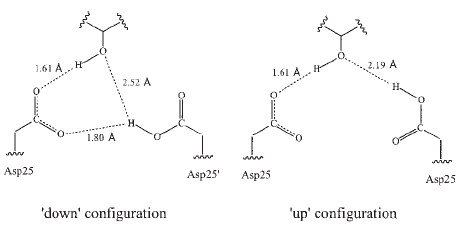
\includegraphics[]{asp_conf}
    \caption{Two conformations of the monoprotonated catalytic aspartic acid dyad of HIV are possible, they are labelled `down' and `up', respectively. The difference between the two lies in the positioning, relative to the ligand of the hydrogen atom. In the `down' position the hydrogen atom is involved in a hydrogen both with the unprotonated Asp25. In the `up' conformation it is involved in a bond with the ligand.}
    \label{fig:asp_conf} 
  \end{center}
\end{figure}

Our reverse transcriptase study indicates the need for simulations of the apo protein we propose to simulate 
10 replica ensembles with 4 ns of production run for the wild type and L100I/K103N double mutant in order to 
replicate the sampling we have achieved for the drug bound systems. 

Our proposed resource requirements are shown in Table \ref{t:hiv_req}.

\begin{table}[h]
\scriptsize
\centering
\begin{tabular}[b]
{|c|c|c|c|c|c|c|}
\hline
\textbf{Sim Description} & \textbf{No. Sims} &
\textbf{No. Cores} & \textbf{Disk} &
\textbf{Code} & \textbf{TG machine} & \textbf{Total SUs}\\
\hline
\multicolumn{7}{|c|}{\textbf{PR Catalytic Asp Study}}\\
\hline
7 PIs - WT PR & 240 & 64 & 250GB & NAMD & Ranger & 276,480 \\
\hline
\multicolumn{7}{|c|}{\textbf{PR Multiple Drug Resistance Study}}\\
\hline
7 PIs - 5 MDR systems & 1750 & 64/48 & 250GB & NAMD & Ranger/Kraken & 2,016,000 \\
\hline
\multicolumn{7}{|c|}{\textbf{RT Drug Resistance Study}}\\
\hline
Apo RT Wildtype & 10 & 192 & 300GB & NAMD & Kraken & 768,000\\
\hline
Apo RT L100I/K103N & 10 & 192 & 300GB & NAMD & Kraken & 768,000\\
\hline
Grand total of SUs required & & & & & & 3,828,480\\
\hline
\end{tabular} \caption{Planned simulations and associated computational requirements.}
\label{t:hiv_req}
\end{table}

\subsubsection{Publications}

[1] Towards High-Throughput, High-Performance Computational Estimation of Binding Affinities for 
Patient Specific HIV-1 Protease Sequences. Owain Kenway, David W. Wright, Helmut Heller, Andre Merzky, Gavin Pringle, Jules Wolfrat, 
Peter Coveney and Shantenu Jha, Accepted for TeraGrid 2011

[2] Resolution of Discordant HIV-1 Protease Resistance Rankings Using Molecular Dynamics Simulations. David W. Wright and Peter V. Coveney, Submitted 2011


\subsection{Project 3b: Predicting the affinity of the EGFR kinase domain for drug inhibitors of lung cancer}

\subsubsection{Progress}

Extensive molecular dynamics (MD) simulations have been performed using the TeraGrid allocation 
for the epidermal growth factor receptor (EGFR). EGFR is a major target for drugs in treating lung 
carcinoma as it promotes cell growth and tumour progression. Using TeraGrid resources, we have done 
two simulations: one is to study changes in drug binding affinities due to cancer mutations, the 
other to address activation mechanism by mutations within the EGFR.

We have performed relative binding affinity calculations using multiple (ensemble) short MD 
simulations. Simulations have been run for two tyrosine kinase inhibitors — AEE788 and Gefitinib — 
complexed with wild-type and 4 mutant EGFRs. 50 replicas were used for each molecular systems to 
ensure the calculated properties are reproducible [3]. In principle, all replicas within a single 
ensemble simulation can easily be run concurrently in one day, thanks to the vast number of cores 
on the TeraGrid supercomputers (Ranger for this work). This makes it possible to accurately rank 
drug binding affinities on clinically relevant timescales. We show that ensemble simulations 
correctly rank the binding affinities for these systems: we report the successful ranking of each 
drug binding to a variety of EGFR sequences and of the two drugs binding to a given sequence. The 
study was published recently in J. R. Soc. Interface [3].

Long timescale simulations have been performed to study the mechanism of activation by 
cancer-causing mutations within EGFR. Structural studies have demonstrated that EGFR exists in an 
equilibrium between catalytically active and inactive forms, and dramatic conformational 
transitions occur during its activation. It is known that EGFR mutations promote such conformational 
changes that affect its activation and drug efficacy. The most common EGFR mutation in lung cancer 
patients is a leucine to arginine substitution at amino acid 858 (L858R). To investigate the changes 
of conformational equilibrium between the active and inactive states, 4 replicas of EGFR were used 
for each conformation, and 200ns molecular dynamics simulations were performed for each replica. 
Using TeraGrid resources, as well as the EU Distributed European Infrastructure for Supercomputing 
Applications (DEISA) allocation, we have performed longer simulations than we initially proposed 
(100ns each). Structural and thermodynamic properties have been extracted from these simulations. 
The thermodynamic stabilities of these two conformations are characterized by free energy landscapes 
estimated from molecular mechanics/Poisson–Boltzmann solvent area calculations. Our study reveals 
that the L856R mutation introduces conformational changes in both states, adjusting the relative 
stabilities of active and inactive conformations and hence the activation of the EGFR kinase [4].

\subsubsection{Future Work}

This project has been completed.

\subsubsection{Publications}
[3] Wan, S.; Coveney, P. V. Rapid and accurate ranking of binding affinities of epidermal growth factor receptor sequences with selected lung cancer drugs. J. R. Soc. Interface 2011, doi: 10.1098/rsif.2010.0609.

[4] Wan, S.; Coveney, P. V. Molecular dynamics simulation reveals structural and thermodynamic features of kinase activation by cancer mutations within the epidermal growth factor receptor. J. Comput. Chem. 2011. doi: 10.1002/jcc.21866.

[5] Marias, K.; Dionysiou, D.; Sakkalis, V.; Graf, N.; Bohle, R.; Coveney, P. V.; Wan, S.; Folarin, A.; Buchler, P.; Reyes, M.; Clapworthy, G.; Liu, E.; Sabcznski, J.; Bily, T.; Roniotis, A.; Tsiknakis, M.; Kolokotroni, E.; Giatili, S.; Veith, C.; Messe, E.; Stenzhorn, H.; Kim, Y.-J.; Zasada, S.; Haidar, A.; May, C.; Bauer, S.; Wang, T.; Zhao, Y.; Marasek, M.; Grewer, R.; Franz, A.; Stamatakos, G. Clinically driven design of multi-scale cancer models: the ContraCancrum project paradigm. Interface Focus 2011, 1, 450.

\section{Project 4: Large-scale molecular dynamics simulations of layered bio-mineral composites}

\subsection{Progress}

The objective of this work is to %calculate the properties of clay platelets immersed in a polymer 
matrix (a nanocomposite system) and to investigate the complex interaction between bio-molecules and 
clay-mineral systems relevant to origins of life and applications to drug delivery. This work is 
supported by UK EPSRC RealityGrid Platform Grant (EP/C536452/1), an EPSRC PhD studentship and the 
UK Technology Strategy Board's NIMES (Q2506L) project.

Since a mineral-mediated origin of life was first hypothesized over sixty years ago, clays have 
played a significant role in origins of life studies. Such studies have hitherto rarely used computer 
simulation to understand the possible chemical pathways to the formation of biomolecules. We have used 
molecular dynamics techniques to carry out large-scale simulations of various 25-mer sequences of 
ribonucleic acid (RNA), in bulk water and with aqueous montmorillonite clay over many tens of 
nanoseconds. The results generated from our simulations, performed on Kraken, are found 
to be in agreement with various experimental observations pertaining to the relative adsorption 
of RNA on montmorillonite in the presence of charge balancing cations. Over timescales of only a 
few nanoseconds, specific RNA sequences fold to characteristic secondary structural motifs, which do 
not form in the corresponding bulk water simulations. Our simulations also show that, in aqueous Ca2+
 environments, RNA can tether to the clay surface through a nucleotide base leaving the 3' end of the 
strand exposed, providing a mechanism for the regiospecific adsorption and elongation of RNA oligomers 
on clay surfaces. This work has been published as Swadling \textit{et al} 2010 [6].%\cite{}.

We have also used molecular dynamics simulations to study the structural stability of three different nucleic acids 
intercalated within a magnesium aluminium layered double hydroxide (LDH) mineral, at varying degrees of 
hydration, and free in aqueous solution. The nucleotides investigated are ribose nucleic acid (RNA), 
deoxyribose nucleic acid (DNA), and peptide nucleic acid (PNA), all in duplex form. Our simulations show 
that DNA has enhanced Watson-Crick hydrogen-bonding when intercalated within the LDH clay layers, compared 
with intercalated RNA and PNA, whilst the reverse trend is found for the nucleic-acids in bulk water. 
The tendency for LDH to alter the stability of the three nucleic acids persists for higher temperature 
and pressure conditions. The uncharged protein backbone of PNA is found to have a detrimental effect on 
the overall stability of the duplex, as it experiences a greatly reduced electrostatic interaction with the 
charged LDH sheets compared to RNA and DNA. Assuming an RNA world, in which RNA preceded the DNA/protein 
world, at some point in time DNA must have taken over the role as the information storage molecule from RNA. 
These results suggest that a mineral based origin of life may have favored DNA as the information-storage 
biomolecule over potentially competing RNA and PNA, providing a route to modern biology from the RNA world.
This work has been submitted for publication [7].

We are also studying the interaction of various single-stranded RNA sequences with anionic clays 
of differing surface charge. All RNA molecules simulated in this study are 25 nucleotides in length and are 
single-stranded. A poly adenine sequence was chosen to compare with the sequence used in experiments 
performed by Ferris \textit{et al.} []. Two further sequences were chosen from the hammerhead ribozyme, as 
they are known  to fold into well-defined secondary structural motifs. Each RNA sequence was simulated with 
three separate layered double hydroxide (LDH) mineral surfaces. The LDHs used differed in composition yielding 
a different surface charge. RNA is shown to adsorb on the LDH surface electrostatically through RNA phosphate 
groups and the LDH Mg2+ charge sites. The adsorption happens rapidly (3-4 ns). The RNA, once adsorbed, is orientated in 
a way that could facilitate the polymerization of the nucleic-acid polymer. Additional monomeric nucleotides 
would arrange in such a way that the phosphate would adsorb to a mineral charge site with the base exposed to 
the aqueous region. The distance between nucleotide monomers, or a monomer and polymer, would be equal to the 
length of the phosphate bond; this would facilitate phosphodiester bond formation in nucleic-acid polymerization.
The simulations for this study are ongoing and a manuscript based on the results is in preparation [8].

\subsection{Future Work}

\subsection{Publications}

[6] Clay Minerals Mediate Folding and Regioselective Interactions of RNA: A Large-Scale Atomistic Simulation Study. J. B. Swadling, P. V. Coveney, and H. C. Greenwell. J. Am. Chem. Soc., 132:13750-13764, 2010.

[7] Stability of Free and Mineral-Protected Nucleic Acids: Implications for the RNA World. J. B. Swadling, P. V. Coveney, and H. C. Greenwell. Submitted, 2011.

[8] The Adsorption of Single-Stranded RNA at Anionic Mineral Interfaces: An Atomistic Simulation Study. J. B. Swadling, P. V. Coveney, and H. C. Greenwell. Manuscript under preparation/simulations ongoing, 2011.




\section{Project 5: Expeditions in Distributed Computing using SAGA}

\subsection{Analysis of Data-Intensive Applications on the TeraGrid}

Next-Generation (gene) Sequencing (NGS) machines produce unprecedented amounts of data.  In addition to the challenge of data-management that arise from unprecedented volumes of data, there exists the important requirement of effectively analyzing large volumes of data.  It is worth mentioning that the computational complexity of the analysis (e.g. mapping) depends, upon other things, the size and complexity of the reference genome \& the data-size of short reads.  Given that these can vary significantly, the computational requirements of NGS-analytics also varies (even between data-sets of similar size).  Thus an efficient, scalable and extensible analytical approaches must be supported by any framework supporting NGS-analytics.

We have created the DARE-NGS Gateway (\url{http://cyder.cct.lsu.edu/dare-ngs}) which supports Genome-wide analysis on the TeraGrid and other distributed cyber-infrastructure.  DARE-NGS builds upon the Distributed Adaptive Runtime-Environment (DARE) Framework, which support a range of tasks with varying computing and data requirements over a wide range of high-performance and distributed infrastructure.  Using DARE-NGS we have analyzed the full Human-Genome (requiring data-sets of upwards of 250GB) on TeraGrid machines such as Ranger. This is work in progress, done entirely in the period of this award period; we are still extending the DARE-NGS capabilities to support other advanced algorithms\cite{ecmls11}.

\subsection{Frameworks for Supporting the Scale-up and Scale-out of Ensembles based Simulations}

In Ref.~\cite{async-re}, we have continued to develop the capabilities to perform arguably the world's largest number of replica-exchange simulations using the SAGA Repex-Framework. Most experiments, validation and refinements have been performed in the award period. Important refinements in the communication and coordination approaches remain, as well as in the ability to scale-out to even more resources/cores. This is the proposed area of activity over the next phase so that several application research groups can use this framework (eg Bishop (Tulane), Ron Levy (Rutgers) and Darrin York (Rutgers)), as well as for Project 2 and 4.

We have used the underlying framework that is being developed and
tested using this allocation, to support the project ``Running Many MD
Simulations on Many Supercomputers'' -- a collaboration with Tom
Bishop as part of Bishop's TRAC award. This work is scheduled for
submission to TeraGrid 2011 Conference (and to Journal of Chemical
Informatics and Modeling).

1

\end{document}
